\usecaseristoratore{Risposta ad un \textit{feedback}}
\label{usecase:Risposta ad un feedback}

\begin{figure}[h]
	\centering
	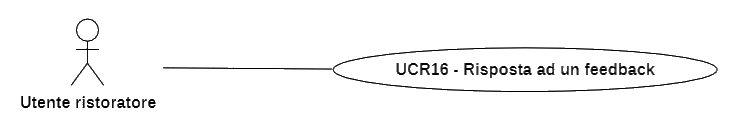
\includegraphics[width=0.8\textwidth]{./uml/UCR16.png} 
	\caption{Risposta ad un \textit{feedback}}
	\label{fig:UCR16}
  \end{figure}

\begin{itemize}
	\item \textbf{Attore principale:} Utente ristoratore.

	\item \textbf{Precondizione:} L'Utente ristoratore è entrato nella sezione di consultazione dei \textit{feedback} relativi al suo ristorante.

	\item \textbf{Postcondizione:} L'Utente ristoratore risponde ad un \textit{feedback} scritto da un Utente base.


	\item \textbf{Scenario principale:}
	      \begin{enumerate}
		      \item L'Utente ristoratore risponde ad un \textit{feedback};
		      \item Il Sistema registra la risposta del ristoratore.

	      \end{enumerate}
\end{itemize}
